\chapter{Metody fingerprintingu urządzeń i przeglądarek}
Od kiedy Eckersley \cite{eckersley2010unique} po raz pierwszy opisał
\emph{fingerprinting} przeglądarek, metody \emph{fingerprintingu} zmieniały się
i ewoluowały razem z nimi. Sytuacja \emph{fingerprintingu} poszczególnych
protokołów czy implementacji stosu TCP/IP jest raczej odmienna. Choć te metody
znane są już od lat dziewięćdziesiątych (a ich implementacje to takie narzędzia
jak nmap), są relatywnie mniej ,,przebojowym'' tematem badań i eksperymentów.
Niniejszy rozdział enumeruje przez szeroką gamę metod, prezentując implementacje
najważniejszych i rozważając ich skuteczność.

\section{Pojęcie pasywnego i aktywnego fingerprintingu}
\emph{Fingerprinting} może być przeprowadzany w sposób pasywny lub aktywny.
Pasywny polega całkowicie na informacjach, do których zdobycia nie jest wymagana
interakcja z drugą stroną połączenia (np. nagłówki HTTP (takie jak
\emph{User-Agent}))---te informacje i tak zostają wysłane. Aktywny
\emph{fingerprinting} opiera się z kolei na przykład na użyciu skryptów do
wydobycia większej ilości informacji (takich jak konfiguracja przeglądarki)
\cite[s. 3]{al2020too}.

\section{Źródła danych identyfikacyjnych}
Mówiąc o warstwach modelu TCP/IP możemy wyróżnić następujące źródła danych (w
kolejności warstw modelu TCP/IP zaczynając od warstwy dostępu do sieci):
\begin{enumerate}
	\item Różnice w implementacjach protokołów (takich jak CDP);
	\item Różnice w implementacjach protokołów (takich jak ICMP);
	\item Różnice w implementacjach stosu TCP/IP;
	\item Różnice w implementacjach protokołów i aplikacji korzystających z
	      nich.
\end{enumerate}

\section{Fingerprinting implementacji stosu TCP/IP}
Jedną z ciekawych właściwości różnic w implementacjach stosu TCP/IP jest fakt,
iż ruch sieciowy z komputera ofiary może być analizowany w celu wykrycia,
jakiego systemu operacyjnego używa (na przykład). Powodem tej sytuacji jest
przeniesienie odpowiedzialności o ustaleniu wartości pewnych parametrów
protokołów TCP i IP na stronę zajmującą się implementacją. Różne wersje tego
samego systemu operacyjnego i różne systemy operacyjne używają różnych wartości
tych parametrów. Może pozwalać to na unikalną identyfikację lub chociaż
oszacowanie jakiego typu technologią jest druga strona połączenia.

% Initial packet size (16 bits); Initial TTL (8 bits); Window size (16 bits);
% Max segment size (16 bits); Window scaling value (8 bits); "don't fragment"
% flag (1 bit); "sackOK" flag (1 bit); "nop" flag (1 bit).

Parametry, które mogą różnić się pomiędzy implementacjami stosu TCP/IP to między
innymi:
\begin{itemize}
	\item początkowy rozmiar pakietu;
	\item początkowy TTL;
	\item szerokość okna;
	\item maksymalna długość segmentu;
	\item wartość progowa, po której okno zaczyna być skalowane;
	\item flagi \emph{don't fragment}, \emph{sackOK} i \emph{nop}.
\end{itemize}
Sumaryczna ilość informacji, które dają wymienione parametry to 67 bitów.
Natomiast Hjelmvik \cite{hjelmvik2011passive} pokazuje, że jedynie nawet
początkowy TTL i szerokość okna wystarczają, aby rozpoznać system operacyjny, z
którego pochodzi analizowany ruch sieciowy (Rys. 3).

\begin{figure}
	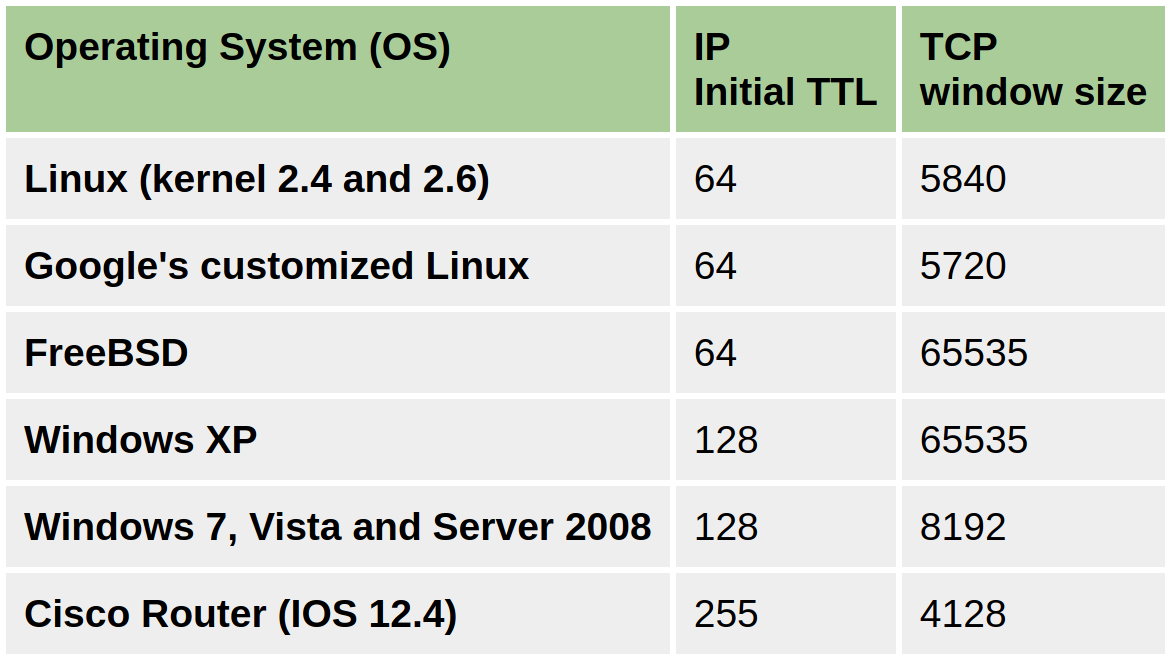
\includegraphics[width=\textwidth,keepaspectratio]{img/03}
	\source{\cite{hjelmvik2011passive}}
	\caption{Różnice w początkowym TTL i szerokości okna pomiędzy systemami}
\end{figure}

\subsection{Opis algorytmu}
O ile analiza ruchu sieciowego i wydobywanie odpowiednich parametrów jest
relatywnie bezpośrednie w przypadku większości z nich, to pewnym problemem jest
początkowa wartość TTL. W przypadku tego parametru host wysyłający pakiet ustawi
wartość równą domyślnej dla danego systemu operacyjnego, ale będzie ona
pomniejszana o jeden dla każdego routera na drodze do hostu docelowego. Zatem
początkową wartością TTL będzie zaobserwowany TTL plus liczba skoków.

\section{Fingerprinting przeglądarek}
Znane metody \emph{fingerprintingu} przeglądarek, które można uznać za
praktycznie stosowane (na przykład będące treścią implementacji popularnych,
otwartoźródłowych bibliotek czy tematem badań nad prywatnością i bezpieczeństwem
komputerowym) to techniki, które polegają na użyciu takich danych jak:
\begin{itemize}
	\item nagłówek User-Agent;
	\item informacja o tym, czy przeglądarka jest tzw.
	      marionetką\footnote{https://developer.mozilla.org/en-US/docs/Web/API/Navigator/webdriver};
	\item język przeglądarki;
	\item głębia koloru ekranu urządzenia;
	\item wielkość RAM urządzenia;
	\item proporcja pomiędzy fizycznymi a logicznymi pikselami ekranu
	      urządzenia;
	\item liczba procesorów logicznych urządzenia;
	\item rozdzielczość ekranu urządzenia;
	\item dostępna rozdzielczość ekranu urządzenia;
	\item przesunięcie strefy czasowej zegara systemowego;
	\item strefa czasowa zegara systemowego;
	\item możliwość dostępu do magazynu \texttt{sessionStorage};
	\item możliwość dostępu do magazynu \texttt{localStorage};
	\item możliwość dostępu do IndexedDB;
	\item możliwość prototypowania \texttt{HTMLElement};
	\item wsparcie dla WebSQL;
	\item klasa procesora urządzenia;
	\item platforma, na której działa przeglądarka;
	\item nagłówek Do Not Track;
	\item zainstalowane \emph{pluginy};
	\item \emph{fingerprint} elementu \texttt{canvas};
	\item \emph{fingerprint} WebGL;
	\item rozszerzenie \texttt{WEBGL\_debug\_renderer\_info};
	\item użycie rozszerzeń blokujących reklamy;
	\item informacja o tym, czy przeglądarka fałszuje język;
	\item informacja o tym, czy przeglądarka fałszuje rozdzielczość ekranu
	      urządzenia;
	\item informacja o tym, czy przeglądarka fałszuje system operacyjny;
	\item informacja o tym, czy przeglądarka fałszuje informacje o sobie;
	\item wsparcie dla interakcji dotykowych przez urządzenie;
	\item lista obsługiwanych czcionek;
	\item lista obsługiwanych czcionek Flash;
	\item \emph{fingerprint}
	      audio\footnote{https://audiofingerprint.openwpm.com/};
	\item lista podłączonych urządzeń peryferyjnych do urządzenia.
\end{itemize}

Zbieranie powyższych danych zostanie szczegółowo omówione w niniejszym
rozdziale.

\subsection{Canvas fingerprinting}
Przeglądarki internetowe są coraz bardziej skomplikowanymi programami
komputerowymi i coraz częściej udostępniają stronom internetowym funkcjonalności
do tej pory oferowane jedynie przez system operacyjny. Pewnym naturalnym
schematem, aby zaimplementować niektóre zaawansowane funkcjonalności
przeglądarek, jest korzystanie z zasobów systemowych i sprzętowych hosta. Na
przykład przetwarzanie grafiki używając karty graficznej, daje ogromny skok
wydajnościowy i bardziej oszczędza baterię w przypadku urządzeń mobilnych. Nie
inaczej jest w przypadku elementu \texttt{canvas}. HTML5 zawiera w sobie
element, na którym można programowo rysować, a użycie natywnych mechanizmów
systemu operacyjnego \emph{renderingu} czcionek do tekstu (na
przykład\footnote{Oczywiście element \texttt{canvas} pozwala na rysowanie
	praktycznie dowolnych rzeczy (obiektów):
	https://developer.mozilla.org/pl/docs/Web/API/Canvas\_API/Tutorial})
gwarantuje, że rezultat będzie zoptymalizowany pod kątem wyświetlania na
konkretnym ekranie i zgodny z oczekiwaniami użytkownika. Ściślejsze powiązanie
przeglądarki internetowej z funkcjonalnością systemu operacyjnego i samym
sprzętem oznacza, że strony internetowe mają większy dostęp do tych zasobów, a
zachowanie przeglądarki różni się w zależności od zachowania tych zasobów
\cite[s. 1]{mowery2012pixel}. Trudno wyobrazić sobie liczbę warstw abstrakcji od
samego sprzętu, przez sterowniki urządzeń i system operacyjny, aż po wyświetlany
efekt na ekranie użytkownika. Im dalej wgłąb tego stosu, tym więcej nieścisłości
uwypukli się, rozważając różne konfiguracje sprzętowe, systemy operacyjne i
przeglądarki internetowe. Z tej prawidłowości został wcześniej w niniejszej
pracy wyciągnięty wniosek, że \emph{fingerprint} urządzenia może zawierać się w
\emph{fingerprincie} przeglądarki.

Analogiczną techniką jest \emph{fingerprinting} WebGL, która także polega na
rysowaniu w elemencie \texttt{canvas} (scen trójwymiarowych).

\subsubsection{Historia}
W 2012 roku Keaton Rowery i Hovav Schacham z Uniwersytetu Kalifornijskiego w San
Diego opublikowali artykuł ,,Pixel Perfect: Fingerprinting Canvas in HTML5''
\cite{mowery2012pixel}, który jako pierwszy poruszył temat Canvas
fingerprintingu. Autorzy określili wówczas tę technikę jako deterministyczną, o
wysokiej entropii, niezależną od innych technik, transparentną (niezauważalną)
dla użytkownika i prostą do zastosowania \cite[s. 1]{mowery2012pixel}.
Podsumowują, że wszystkie nowe możliwości przeglądarek internetowych mają swój
koszt \cite[s. 3]{mowery2012pixel}. Ich eksperymenty polegały głównie na
rysowaniu tekstu w elemencie \texttt{canvas} i pokazały, że co najmniej używany
system operacyjny, wersja przeglądarki, karta graficzna, zainstalowane czcionki,
hinting czcionek na poziomie subpiksela, antyaliasing, a nawet konkretne
ułożenie pikseli na fizycznym ekranie (coś, co mogą brać pod uwagę takie
technologie jak ClearType) grają role w generowaniu bitmapy z elementu
\texttt{canvas}. Nawet czcionka Arial, która ma ponad 30 lat renderowała się
,,na nowe i interesujące sposoby'' w eksperymentach \cite[s.
6]{mowery2012pixel}. Canvas fingerprinting rozgłos zdobył jednak dopiero po
publikacji ,,The Web Never Forgets: Persistent Tracking Mechanisms in the Wild’’
z 2014 roku \cite{acar2014web}. Wtedy o Canvas fingerprintingu pisały wszystkie
największe media na świecie.

\subsubsection{Pseudokod}
\begin{algorithm}[H]
	\SetAlgoVlined
	\SetAlgoCaptionSeparator{.}
	\SetKwInOut{Input}{Dane}
	\SetKwInOut{Output}{Wynik}
	\SetKwData{Canvas}{canvas}
	\SetKwData{Ctx}{ctx}
	\SetKwData{TwoD}{2d}
	\BlankLine
	\Input{Element \Canvas}
	\Output{Reprezentacja graficzna elementu \Canvas}
	\BlankLine
	\If{przeglądarka obsługuje wybranie kontekstu graficznego}{
		\Ctx $\leftarrow$ jeden z kontekstów graficznych, np. \TwoD\;
		\tcp{użycie \Ctx, aby wpłynąć na element \Canvas}
		\If{przeglądarka obsługuje pakowanie elementu \Canvas}{
			\Return{reprezentacja elementu \Canvas}\;
		}
		\Return{informacja o braku możliwości wykonania algorytmu}\;
	}
	\Return{informacja o braku możliwości wykonania algorytmu}\;
	\caption{Canvas fingerprinting}
\end{algorithm}

\subsubsection{Implementacja w JavaScript}

\subsection{Audio fingerprinting}

\subsection{Pozostałe techniki}

% \subsection{Protokoły warstwy drugiej w modelu OSI}

% \subsection{Stos TCP/IP}

% \subsubsection{Protokoły warstwy 3 i 4 w modelu OSI}

% \paragraph{IPv4}

% \paragraph{IPv6}

% \paragraph{ICMP}

% \paragraph{IEEE802.11}

% \subsection{Nierutowalne protokoły warstwy 5 (lokalny fingerprinting)}

% \subsection{Rutowalne protokoły warstwy 7}

% \section{Wybrane metody fingerprintingu urządzeń i ich systemów operacyjnych}

% \section{Przeglądarki jako specjalny przypadek fingerprintingu urządzeń}

% \section{Źródła danych identyfikacyjnych przeglądarek}

% \section{Wybrane metody fingerprintingu przeglądarek}

% \subsection{Implementacje wybranych metod fingerprintingu przeglądarek}

% \section{Implementacja przykładu identyfikacji przeglądarki}
